\subsection{SP-17 (OSY)}
Procesy a vlákna, jejich implementace, nástroje pro synchronizaci vláken. Klasické synchronizační úlohy. Uváz\-nu\-tí (deadlock) vláken (alokace prostředků, Coffmanovy podmínky, strategie pro řešení uváznutí).

\begin{itemize}
	\item \textbf{Program:} 
	
	Program je v systému reprezentován spustitelným binárním programem, který je uložený v sekundární paměti (např. disk).
	
	\item \textbf{Proces:} 
	
	Instance spuštěného programu/aplikace. Entita, v rámci které jsou alokovány prostředky (paměť, vlákna, otevřené soubory, zámky, semafory, sokety,...).
	
	\item \textbf{Vlákno:} 
	
	Výpočetní entita (proud instrukcí), které je přidělováno jádro CPU. Vlákna vytvořená v rámci procesu sdílí většinu prostředků alokovaných v tomto procesu.
\end{itemize}

\textbf{Vytvoření procesu:}

Nový proces lze vytvořit jako kopii/klon původního procesu, či jako úplně nový proces. V Unixu fork() exec(), ve Windows CreateProcessA().

\begin{itemize}
	\item \textbf{fork():}
	
	Vytvoří nový proces, který je kopií toho procesu, ze kterého byla tato funkce zavolána. V případě chyby vrací -1, v potomkovi vrací 0, v rodiči vrací PID potomka.
	
	\item \textbf{exec():} 
	
	Adresový prostor aktuálního procesu je přepsán obsahem souboru, který se začne vykonávat od začátku.
	
	\item \textbf{wait():} 
	
	Zablokuje rodičovský proces, ve kterém je zavolána, dokud se konkrétní/jeden potomek neukončí.
\end{itemize}

\textbf{Ukončení procesu:}
\begin{itemize}
	\item jádro se pokusí předat návratový kód rodiči
	\item ukončí se všechna vlákna pod procesem
	\item uvolní se adresový prostor procesu a příslušné struktury OS
	\item proces se může ukončit sám (buď normální konec programu jako \textit{return}, nebo chyba, kvůli které se sám ukončí), nebo může být ukončen jádrem (fatální chyba nebo signál od jiného procesu)
\end{itemize}

\textbf{Vlákna:}
\begin{itemize}
	\item proces se implicitně vytváří s jedním "main" vláknem
	\item další vlákna lze vytvořit z hlavního (volání OS)
\end{itemize}

\textbf{Plánování:} 
\begin{itemize}
	\item vláken je typicky zásadně více než logických jader procesoru
	\item jedno vlákno je zpracováváno max 1 logickým jádrem
	\item aby se vlákna na jádrech vystřídala, používá se typicky preemptivní plánování
	\begin{itemize}
		\item vlákno je na základě plánovacích kritérií vybráno, a je mu přiděleno volné jádro CPU
		\item vláknu je přiděleno množství času na CPU
		\item vláknu je jádro odebráno, pokud uplyne přidělený čas, vlákno provede systémové volání nebo dojde k přerušení
	\end{itemize}
	\item přepínání kontextu (vystřídání vláken na jádře CPU)
	\begin{itemize}
		\item kontext = všechny nezbytné informace pro pozdější spuštění přerušeného vlákna od okamžiku pře\-ru\-še\-ní
		\item kontext se uloží do paměti, naplánuje se další vlákno a jeho kontext se nahraje do CPU jádra
	\end{itemize}
\end{itemize}

\textbf{Stavy vláken:}

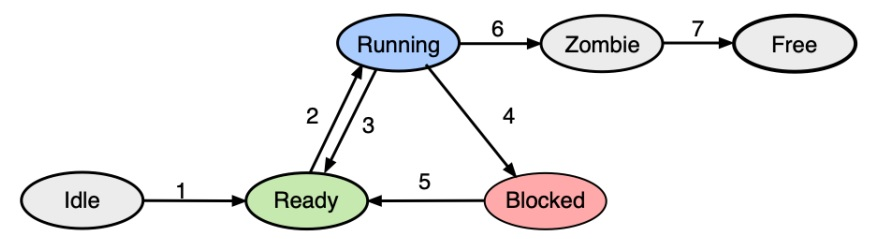
\includegraphics[width=0.8\textwidth]{img/SP-17_0.jpg}

\begin{itemize}
	\item \textbf{Časově závislé chyby:}
	
	Situace, kdy více vláken používá společné sdílené prostředky a výsledek deterministického algoritmu je závislý na rychlosti jednotlivých vláken, které používají tyto prostředky. Špatně se detekují --- lze předcházet správným návrhem paralelního algoritmu.
	
	\item \textbf{Kritická sekce:}
	
	Část programu, kde vlákna používají sdílené prostředky.
	
	\item \textbf{Sdružené kritické sekce:}
	
	Kritické sekce více vláken, které se týkají stejného sdíleného prostředku.
	
	\item \textbf{Vzájemné vyloučení:}
	
	Vláknům není dovoleno sdílet stejný prostředek ve stejném čase, tedy se nenachází ve stejné sdružené sekci současně.
	
	\item \textbf{Korektní paralelní program:}
	
	Nesmí klást předpoklady na rychlost vláken a počet jader. Musí zajistit výlučný přístup ke sdíleným prostředkům. Mimo kritické sekce by vlákno nemělo být zpomalováno ostatními vlákny.
\end{itemize}

\textbf{Problémy s použitím synchronizace vláken:}
\begin{itemize}
	\item deadlock (x vláken čeká na událost, kterou může vyvolat jen jedno z čekajících vláken)
	\item livelock (několik vláken vykonává neužitečný výpočet, ale nemohou dokončit)
	\item starvation (vlákno ve stavu "ready" předbíháno a dlouho se nedostane na řadu)
\end{itemize}

\textbf{Zamykání kritických sekcí:}
\begin{itemize}
	\item zámek značí, zda je ve sdružené kritické sekci už jiné vlákno --- musí se k němu přistupovat atomicky (např. TSL --- Test and Set Lock)
	\item aktivní vs blokující čekání
\end{itemize}

\begin{itemize}
	\item \textbf{Zámek (mutex):}
	
	Pamatuje si svůj stav (zamčený/odemčený) a množinu vláken blokovaných na něm. Jsou nad ním definovány atomické operace lock() a unlock().
	
	\item \textbf{Podmíněná proměnná (conditional variable):}
	
	Pamatuje si, která vlákna jsou na ní blokována. jsou definovány operace cond\_wait(mutex) a cond\_signal(). cond\_wait(mutex) --- mutex musí být zamčen volajícím vláknem, funkce odblokuje mutex a zablokuje vlákno dokud nepřijde cond\_signal().
	
	\item \textbf{Semafor:}
	
	Obsahuje čítač a seznam blokovaných vláken. Jsou definovány operace sem\_init(int) (nastaví čítač na 0), sem\_wait() (vstup do sekce --- pokud čítač je větší než 0 tak vlákno vstoupí a dekrementuje čítač, jinak se zablokuje) a sem\_post() (uvolní nějaké čekající vlákno, nebo inkrementuje čítač).
	
	\item \textbf{Bariéry:}
	
	Obsahuje čítač (síla bariéry --- kolik vláken musí čekat, aby byla odblokována) a blokovaná vlákna. Operace: barrier\_init(int) (nastaví sílu bariéry) a barrier\_wait() (pokud čítač je více než 1, vlákno čeká a čítač je dekrementován, jinak jsou všechna vlákna probuzena)
	
\end{itemize}

\textbf{Synchronizační úlohy:}
\begin{itemize}
	\item Večeřící filosofové
	\begin{itemize}
		\item $N$ filosofů u kulatého stolu
		\item každý má před sebou jídlo a mezi sousedními talíři je vždy 1 vidlička (celkem tedy $N$ vidliček)
		\item pokud chce filosof jíst, musí získat obě vidličky vedle jeho talíře
		\item stavy filosofa: přemýšlí (nechce a nemá vidličky), má hlad (pokouší se získat obě vidličky), jí (má obě vidličky)
		\item optimální řešení: může jíst až $\lfloor N/2 \rfloor$ filosofů, nevznikají časově závislé chyby ani synchronizační problémy
		\item řešení: pokud mam hlad zamknu mutex, kouknu jestli jsou volny vidlicky, pokud ne spim (odemykam mutex), pokud jo, beru, odemykam mutex a jim. Az dojim, zamknu mutex, vratim vidlicky, probudim sousedy a odemknu mutex.
	\end{itemize}
	
	\item Čtenáři --- písaři
	\begin{itemize}
		\item v systému je 1 sdílený prostředek
		\item písaři mohou modifikovat, čtenáři pouze číst
		\item chceme, aby pokud není modifikováno (nepřistupuje písař) mohlo číst více čtenářů
		\item zároveň by nikdo neměl být předbíhán
		\item řešení: písaři i čtenáři se řadí do fronty, ale po skupinách --- pokud přijdu na konec fronty a je tam už stejný typ, přidám se do skupiny --- na začátku fronty je probuzena celá skupina a buď písaři postupně zapíšou, nebo čtenáři společně přečtou
	\end{itemize}
	
	\item Spící holiči
	\begin{itemize}
		\item v holičství je $N$ holičů a křesel k holení, a $M$ křesel k čekání
		\item pokud nejsou zákazníci, holič sedne do holícího křesla a usne
		\item pokud přijde zákazník, buď probudí holiče (pokud je volný), nebo si sedne do čekárny (pokud je místo) jinak odejde
	\end{itemize}
\end{itemize}

\textbf{Obecně alokace prostředku:}
\begin{itemize}
	\item vlákno žádá o prostředek pomocí alokační funkce
	\item pokud je prostředek volný, je přidělen
	\item pokud je již alokovaný, vlákno může být blokováno (v závislosti na alokační funkci --- mutex\_lock blokuje, mutex\_try\_lock blokuje jen na určitý čas, fork() a malloc() neblokují)
	\item v případu 2 a 3 se vlákno pak samo rozhodne jak pokračovat
\end{itemize}

\textbf{Coffmanovy podmínky}

Uváznutí (deadlock) nastane pouze pokud jsou splněny všechny následující podmínky:
\begin{itemize}
	\item Vzájemné vyloučení --- každý prostředek nemůže být sdílen více vlákny
	\item Podmínka neodnímatelnosti --- již přidělený prostředek nemůže být odebrán násilím
	\item Podmínka "drž a čekej" --- vlákno s již přiděleným prostředkem může žádat o další
	\item Podmínka kruhového čekání --- musí existovat smyčka více vláken, ve které každé vlákno čeká na prostředek držený dalším vláknem ve smyčce
\end{itemize}

\textbf{Řešení uváznutí:}
\begin{itemize}
	\item Pštrosí strategie --- ignorování
	\item Prevence uváznutí --- nesplnění alespoň jedné z Coffamnových podmínek
	\item Předcházení vzniku uváznutí --- pečlivá alokace prostředků
	\item Detekce uváznutí a zotavení --- uváznutí je detekováno a odstraněno
\end{itemize}

\textbf{Implementace procesů:}
\begin{itemize}
	\item jádro OS si udržuje zřetězený seznam struktur --- tabulku procesů
	\item jedna položka tabulky obsahuje vše nezbytné, co si OS musí o procesu pamatovat (PCB --- Process Control Block)
	\begin{itemize}
		\item identifikace procesu (id procesu, id rodiče, číslo úlohy/seance/projektu, jméno procesu...)
		\item identita/bezpečnost (vlastník, skupiny, práva procesu)
		\item informace o alokovaných prostředcích (paměť, soubory, prostředky pro meziprocesovou komunikaci)
	\end{itemize}
\end{itemize}

\textbf{Implementace vláken:}
\begin{itemize}
	\item Thread Control Block (TCB) --- identifikace vlákna, info o přepínání kontextu (registry), informace pro plánování vláken
	\item Implementace v uživatelském prostoru (zastaralé)
	\begin{itemize}
		\item OS přistupuje k procesům jako by měly jedno vlákno
		\item proces si svá vlákna spravuje sám
		\item kooperativní plánování pro vlákna v procesu
	\end{itemize}
	\item Implementace v jádře OS
	\begin{itemize}
		\item OS plánuje samotná vlákna, ne procesy
		\item OS udržuje jede PCB pro každý proces, jeden TCB pro každé vlákno
		\item preemptivní plánování pro vlákna v procesu
	\end{itemize}
\end{itemize}

\textbf{Plánování v dnešních OS:} Prioritní Round Robin

$X$ front s různou prioritou. Na základě předchozího běhu vlákna se buď zvýší časové kvantum a sníží priorita (pokud vlákno využilo všechen čas) nebo zvýší priorita a sníží čas (pokud nevyužilo celé časové kvantum).